\documentclass[14pt]{beamer}
\setbeamertemplate{itemize item}{$\bullet$}
\setbeamertemplate{navigation symbols}{}
\setbeamertemplate{mini frames}{}
\setbeamertemplate{section in toc}[sections numbered]
\setbeamertemplate{itemize items}[square]
\setbeamercolor*{item}{fg=gray}
\usecolortheme{dove}
\hypersetup{pdfpagemode=FullScreen}

\usepackage[yyyymmdd]{datetime}

% Define some accent colors:
\definecolor{DarkFern}{HTML}{407428}
\definecolor{DarkCharcoal}{HTML}{4D4944}
\colorlet{Fern}{DarkFern!85!white}
\colorlet{Charcoal}{DarkCharcoal!85!white}
\colorlet{LightCharcoal}{Charcoal!50!white}
\colorlet{AlertColor}{orange!80!black}
\colorlet{DarkRed}{red!70!black}
\colorlet{DarkBlue}{blue!70!black}
\colorlet{DarkGreen}{green!70!black}
\definecolor{palecerulean}{rgb}{0.61, 0.77, 0.89}

% Use the colors:
\setbeamercolor{alerted text}{fg=palecerulean}
\setbeamercolor{title}{fg=blact}

% Create horizontal rule, header, and title page
\makeatletter
\def\vhrulefill#1{\leavevmode\leaders\hrule\@height#1\hfill \kern\z@}
\makeatother
\setbeamertemplate{frametitle}{\color{black}\bfseries\insertframetitle\par\vskip-6pt\color{palecerulean}\vhrulefill{1.75pt}}
\defbeamertemplate*{title page}{customized}[1][]
{
	{\begin{centering}
	\usebeamerfont{title}\bfseries\inserttitle\par\bigskip
	\usebeamerfont{subtitle}\insertsubtitle\par\vskip-3pt\color{palecerulean}\vhrulefill{1.75pt}\color{black}\\
	\bigskip
	\bigskip
	\usebeamerfont{author}\insertauthor\par\bigskip
	\usebeamerfont{institute}\insertinstitute\par
	\usebeamerfont{date}\insertdate\par
	\usebeamercolor[fg]{titlegraphic}\inserttitlegraphic
				\insertframetitle\par
	\smallskip\end{centering}}
}


\title{Immigrant Sentiment and Labour Market Vulnerability}
\subtitle{Economic Perceptions of Immigration in Dualized Labour Markets}
\author{Anthony Kevins\textsuperscript{1} \& Naomi Lightman\textsuperscript{2}}
\institute{\textsuperscript{1}School of Governance, Utrecht 		University\\
	\textsuperscript{2}Department of Sociology, University of Calgary \bigskip}
	\date{June 20, 2019}

\begin{document}

\begin{frame}
\titlepage
\end{frame}

\begin{frame}
	\frametitle{Introduction}
	Immigration tied to numerous economic fears: 
	\begin{itemize}
		\pause
		\item Immigrants take away ``our'' jobs 
		\pause
		\item Immigrants drive down wages 
		\pause
		\item Immigrants drain public coffers	
	\end{itemize}
	\bigskip
	\pause 
	\textbf{Research Question:} What role do economic insecurity and resource scarcity play in shaping these attitudes within and across countries? 
\end{frame}

\begin{frame}
	\frametitle{Background}
	Build from three research areas:
	\begin{enumerate}
		\pause
		\item Individual Perceptions of the Economic Contribution of Immigrants
		\begin{itemize}
			\pause
			\item \textit{Human capital:} low-skill/education levels associated with anti-immigrant attitudes
		\end{itemize}
		\pause
		\item Impact of National Economic Circumstances on Attitudes Towards Immigration
		\begin{itemize}
			\pause
			\item \textit{Resource scarcity:} lower GDP and/or higher unemployment rates associated with anti-immigrant attitudes
		\end{itemize}
		\pause
		\item Dualization and labour market vulnerability  
		\begin{itemize}
			\pause 
			\item \textit{Precarity:} labour market risk increases economic insecurity, even holding related measures (e.g. skill, education, income) constant
		\end{itemize}
	\end{enumerate}
\end{frame}

\begin{frame}
	\frametitle{Hypotheses}
	\begin{itemize}
		\item H1: Greater outsiderness $\rightarrow$ more negative attitudes toward the economic contribution of immigrants 
		% Outsiders view immigrants as disproportionately worsening their already relatively weak labour market position 
		\pause
		\item H2: Higher unemployment rates $\rightarrow$ stronger impact of labour market vulnerability on attitudes toward the economic contribution of immigrants 
		% Sense of resource competition should be greater among outsiders, given that their labour market position is (by definition) less secure
		\pause
		\item H3: Higher GDP $\rightarrow$ stronger impact of labour market vulnerability on attitudes toward the economic contribution of immigrants 
		% In less-developed economies, the general population – not just outsiders – may experience a heightened sense of resource scarcity, leading both insiders and outsiders to feel economically threatened by immigrants; in stronger economies, however, these concerns may be limited to the more vulnerable segments of the labour market
		\pause
		\item H4: Higher GDP $\rightarrow$ weaker impact of labour market vulnerability on attitudes toward the economic contribution of immigrants 
		% Higher levels of GDP per capita might lead everyone in society to be less concerned about resource scarcity, in the process reducing the perceived economic threat from immigrants for the entire population (ignores resource scarcity, but in line with some past research e.g. Pichler, 2010)
	\end{itemize}
\end{frame}

\begin{frame}
	\frametitle{The Survey Data}
	\begin{itemize}
		\item Rounds 4-7 of the European Social Survey (2008, 2010, 2012, and 2014)
		\pause
		\item 23 European countries, 57051 respondents 
		\pause
		\item Dependent Variable:
		\begin{itemize}
			\pause
			\item Would you say it is generally bad or good for [country]’s economy that people come to live here from other countries?
			\pause
			\item 11-point scale ranging from ``bad for the economy'' (0) to ``good for the economy'' (10)
		\end{itemize}
	\end{itemize}
\end{frame}

\begin{frame}
	\frametitle{Measuring Labour Market Vulnerability}
	\begin{itemize}
		\item European Union Statistics on Income and Living Conditions micro-data
		\pause
		\item Continuous ``outsiderness'' scores (Schwander and Häusermann 2013) 
		\begin{enumerate}
			\pause
			\item Parse respondents into subgroups based on occupation, gender, age, and country
			\pause
			\item Calculate mean subgroup rates of temporary contracts, involuntary part-time status, and unemployment
			\pause
			\item Subtract from corresponding country means 
			\pause
			\item Average the three standardized deviation scores
			\pause
			\item Apply value to subgroup members in ESS
			%Also confirm results are robust to small changes, i.e. changing age cut-offs and adding an additional foreign/native-born division
		\end{enumerate}
	\end{itemize}
\end{frame}

\begin{frame}
	\frametitle{Research Design}
	\begin{itemize}[<+-| alert@+>]
		\item<1-> \alert<+>{DV:} Perceived impact of immigrants on the economy
		\item<2-> \alert<+>{Explanatory variables:} outsiderness scores, independently and interacted with GDP (PPP) and national unemployment rates
		\item<3-> \alert<+>{Key individual-level controls:} factors related to precarity (e.g. education, union membership, labour market status, income decile)
		\item<4-> \alert<+>{Country-level controls:} changes in GDP, \% of foreign-born population, and \% of migrant population with tertiary education
	\end{itemize}
\end{frame}

\begin{frame}
	\frametitle{Distribution}
	\begin{figure}
		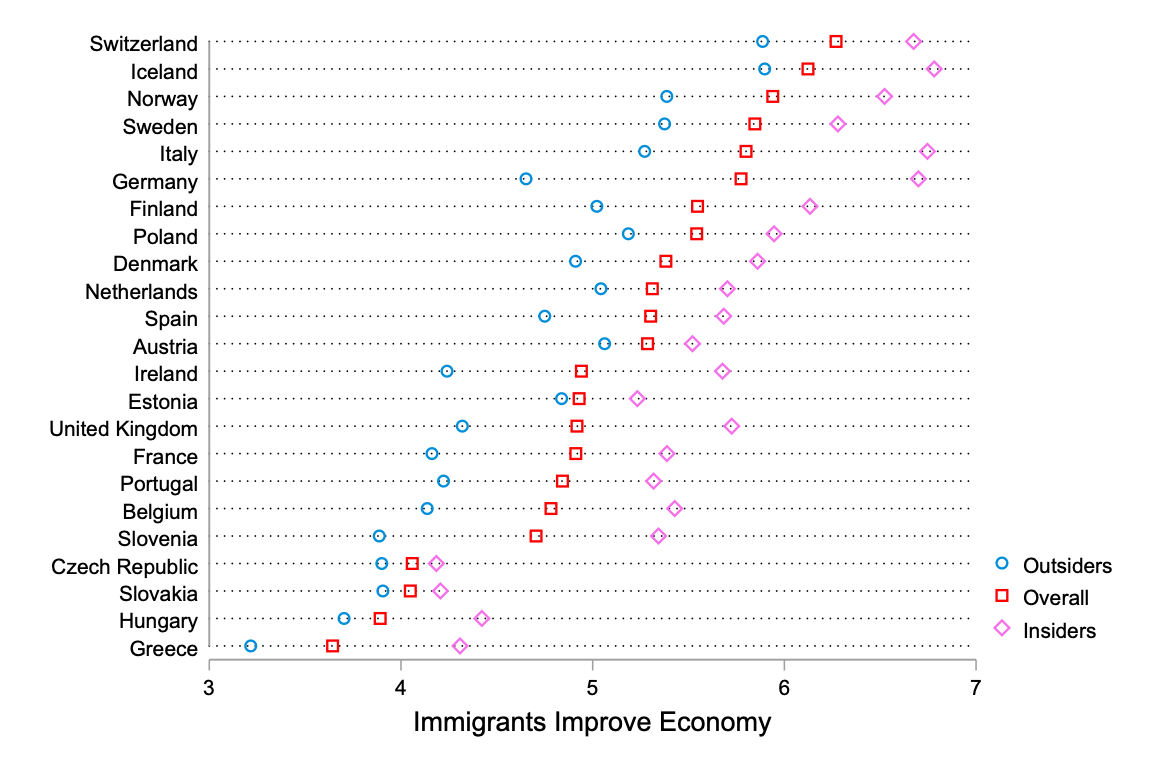
\includegraphics[width=\textwidth]{Figure_1}
		%One SD below and above country means
	\end{figure}
\end{frame}

\begin{frame}
	\frametitle{Marginal Effect of Outsiderness}
	\begin{figure}
		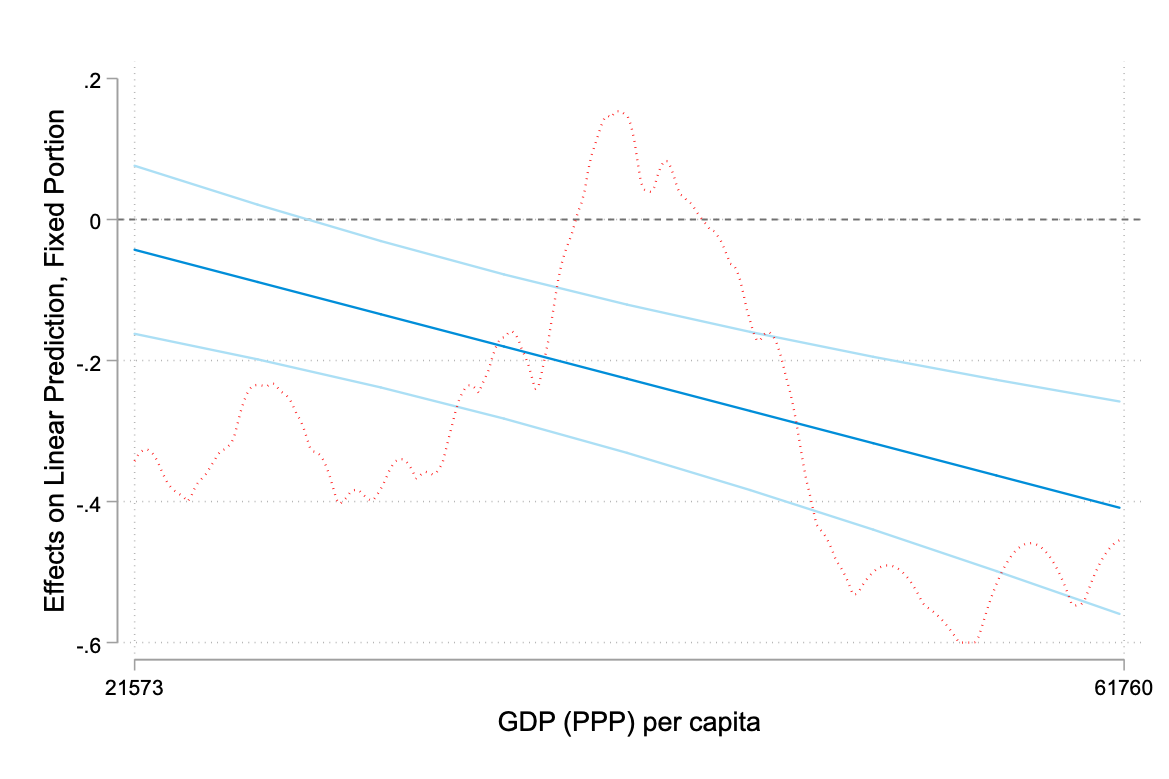
\includegraphics[width=\textwidth]{Figure_2}
		%Exclude bottom/top 5% of GDP values
	\end{figure}
\end{frame}

\begin{frame}
	\frametitle{Linear Prediction}
	\begin{figure}
		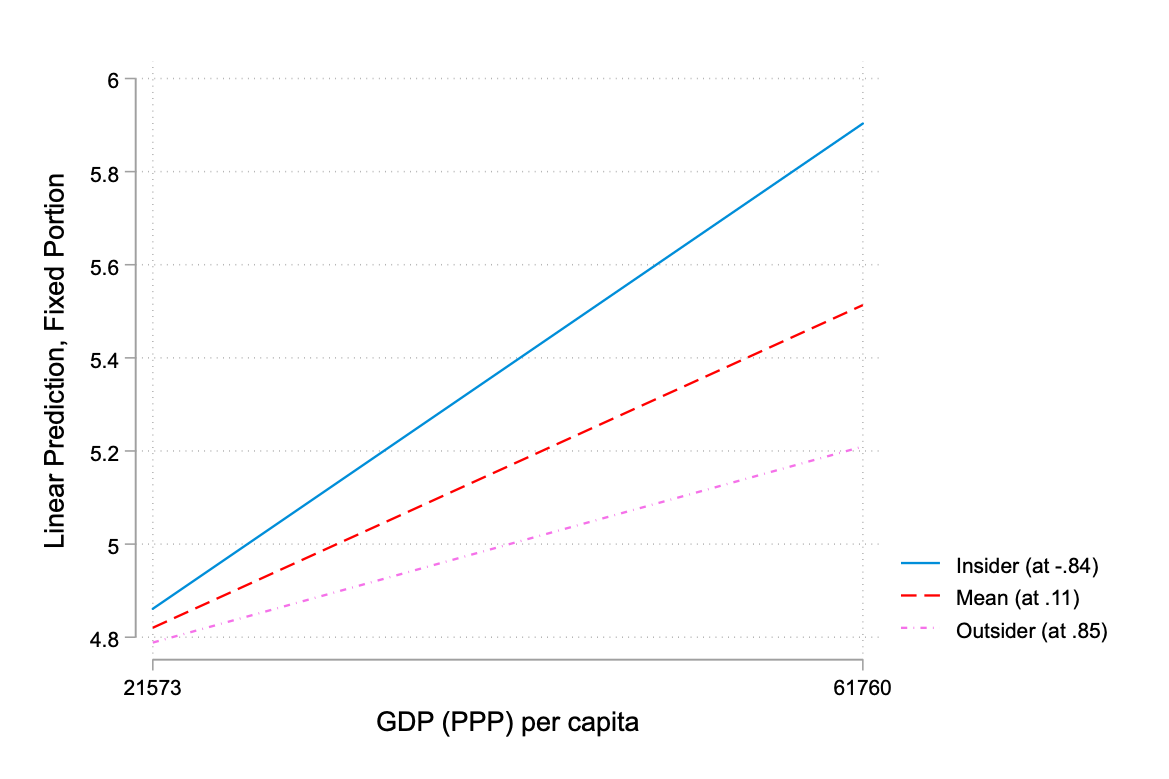
\includegraphics[width=\textwidth]{Figure_3}
		%Alternative visualization: insider at 10th percentile, outsider at 90th
	\end{figure}
\end{frame}

\begin{frame}
	\frametitle{Conclusions}
	Overall findings:
	\begin{itemize}
		\pause
		\item Labour market vulnerability correlated with more negative beliefs 
		\pause
		\item No evidence of an interaction between vulnerability and national unemployment rates
		\pause
		\item Significant interaction between vulnerability and GDP
		\begin{itemize}
			\pause
			\item Labour market insiders and outsiders hold more distinct attitudes in higher GDP countries
		\end{itemize}
	\end{itemize}
\end{frame}

\end{document}
